\documentclass[article, backcover, french, nodocumentinfo]{upmethodology-document}
% Encoding
	\usepackage[utf8]{inputenc}
	%\usepackage[latin1]{inputenc}
	\usepackage[T1]{fontenc}

% Language
	%\usepackage[francais,english]{babel} % Second language = main language

% Show a summary of the layout of the current document with \layout.
	%\usepackage{layout}

% For easy management of document margins and the document page size.
	%\usepackage[top=2cm, bottom=1.8cm, left=1.8cm, right=1.8cm, head=14pt, foot=36pt]{geometry}

% Lets you change line spacing.
	%\usepackage{setspace}

% Euro symbol
	%\usepackage{eurosym}

% Fonts (include only one)
	%\usepackage{bookman}
	%\usepackage{charter}
	%\usepackage{newcent}
	\usepackage{lmodern}
	%\usepackage{mathpazo}
	%\usepackage{mathptmx}

% Enables typesetting of hyperlinks
	%\usepackage{url}
	\usepackage{hyperref}

% Verbatim environment
	%\usepackage{verbatim}
	%\usepackage{moreverb}
	\usepackage{fancyvrb}

% Code listing
	\usepackage{listings}

% To change header and footer of any page of the document.
	\usepackage{fancyhdr}

% Allows you to insert graphic files within a document.
	%\usepackage{graphicx}

% Allows figures or tables to have text wrapped around them.
	%\usepackage{wrapfig}

% Adds support for colored text.
	\usepackage{xcolor}

% Allows tables rows and columns to be colored, and even individual cells.
	%\usepackage{colortbl}

% Mathematics
	\usepackage{amsmath}
	\usepackage{amssymb}
	\usepackage{mathrsfs}
	%\usepackage{asmthm}
	%\usepackage{mathtools}
	%\usepackage{bm} % Greek letters in math mode

% Provide the array and tabular environments
	\usepackage{array}

% Provides control over the layout of the three basic list environments: enumerate, itemize and description.
	%\usepackage{enumitem}

% Interface to sectioning commands for selection from various title styles
	%\usepackage[nobottomtitles]{titlesec}

% Highly customized stacking of objects, insets, baseline changes, etc.
	\usepackage{stackengine}

% Routines for constrained scaling and stretching of objects, relative to a reference object or in absolute terms
	\usepackage{scalerel}

% Provides control over the typography of the Table of Contents, List of Figures and List of Tables, and the ability to create new ‘List of ...’.
	%\usepackage{tocloft}
	%\usepackage{titletoc}

% Advanced bibliography handling.
	%\usepackage{bibtex}
	%\usepackage{biblatex}

% Allows customization of appearance and placement of captions for figures, tables, etc.
	%\usepackage{caption}

% Provides the multicols environment which typesets text into multiple columns.
	%\usepackage{multicol}

% This package simplifies the insertion of external multi-page PDF or PS documents.
	%\usepackage{pdfpages}

% Prints out all index entries in the left margin of the text.
	%\usepackage{showidx}

% It allows to define multiple floats (figures, tables) within one environment giving individual captions and labels in the form 1a, 1b.
	%\usepackage{subcaption}

% Lets you insert notes of stuff to do with the syntax \todo{Add details.}.
	%\usepackage{todonotes}

% Text Companion fonts, which provide many text symbols (such as baht, bullet, copyright, musicalnote, onequarter, section, and yen), in the TS1 encoding.
	\usepackage{textcomp}


% For more information about UPmethodology: https://www.ctan.org/pkg/upmethodology

%=======================================================================================================
%=============================================== Informations ==========================================
%=======================================================================================================

%%% Document Information and Declaration
\declaredocument{Simulation d'un système de livraison par drone}{Projet de LO41}{---}

%%% Abstract and Key-words
\setdocabstract[french]{Projet UTBM de l'UV LO41 du semestre de printemps 2017}
\setdockeywords[french]{UTBM, LO41, drone, delivery, system}

%%% Document Authors and Validators
\addauthorvalidator*[jerome.boulmier@utbm.fr]{Jérôme}{Boulmier}{Étudiant en INFO02}
\addauthorvalidator*[maxime.pinard@utbm.fr]{Maxime}{Pinard}{Étudiant en INFO02}

%%% Informed People
\addinformed*[philippe.descamps@utbm.fr]{Philippe}{Descamps}{Professeur de l'UV LO41}

%%% Copyright and Publication Information
\setcopyrighter{Jérôme Boulmier et Maxime Pinard}
\setpublisher{Jérôme Boulmier et Maxime Pinard}
\setprintingaddress{France}

%%% Version
\incversion{\makedate{\the\day}{\the\month}{\the\year}}{Initial version.}{\upmpublic}

%=======================================================================================================
%================================================== Configs ============================================
%=======================================================================================================

% Change Front Page Layout
%\setfrontcover{modern} % modern or classic

% Change Illustration Picture
%\setfrontillustration[1.3]{figures/figure}

% Source code formatting
\upmcodelang{cpp} % uml, java or cpp

% Prevent page breaks in paragraphs
\predisplaypenalty=1000
\postdisplaypenalty=1000
\clubpenalty=1000

% Minimal space required in the bottom margin not to move the title on the next page
%\renewcommand{\bottomtitlespace}{.1\textheight}

% Links config, especialy for the table of contents
\hypersetup{
    colorlinks=true,
    linkcolor=black,
    urlcolor=blue,
    linktoc=all
}

% French language config
\frenchbsetup{StandardLayout=true,ReduceListSpacing=false,CompactItemize=false}

%=======================================================================================================
%================================================= Functions ===========================================
%=======================================================================================================

%Paragraph with line break
\newcommand{\p}[1]{\paragraph{#1\\}}

% Function to print a warning sign
\newcommand{\dangersign}[1][2.5ex]
	{\renewcommand{\stacktype}{L}
		{\scaleto{\stackon[1pt]{\color{red}$\triangle$}{\fontsize{4pt}{4pt}\selectfont !}}{#1}}}

% Definition of some dt/dx/dy shortcuts for integrals
\newcommand{\dt}
{\;\mathrm{d}\,t}

\newcommand{\dx}
{\;\mathrm{d}\,x}

\newcommand{\dy}
{\;\mathrm{d}\,y}

% Definition of \Witem for 'itemize' environment with a warning sign
\newcommand{\Witem}
{\item[\dangersign{}]}

% Definition of a Max function shortcut
\newcommand{\Max}[2][ ]
{\underset{#1}{\text{Max}}\,#2}

% Definition of a Min function shortcut
\newcommand{\Min}[2][ ]
{\underset{#1}{\text{Min}}\,#2}


\newcommand{\TODO}[2][ ]{\todo[inline,color=green]{#2}}

\begin{document}
	\upmdocumentsummary{}
	\upmdocumentauthors{}
	%\upmdocumentvalidators{}
	\upmdocumentinformedpeople{}
	\upmpublicationpage{}
	\thispagestyle{empty}
	\tableofcontents{}
	%\lstlistoflistings{}
	%\listoffigures{}
	\newpage{}
	\section{Conception}
		\subsection{Réseau de Petri}
			\begin{figure}[H]
			  \centering
			  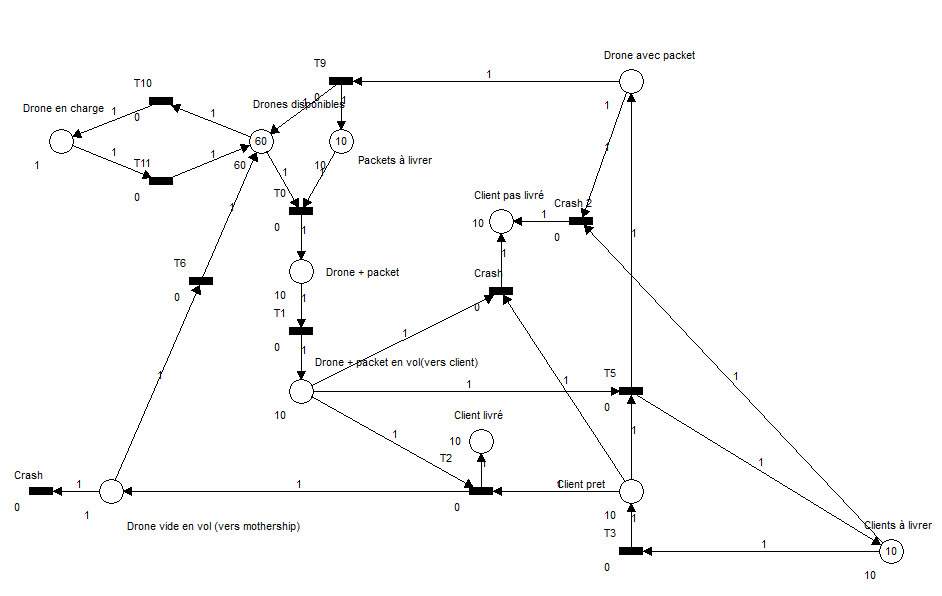
\includegraphics[width=\textwidth]{figures/petri_drones}
			  \caption{Réseau de Petri}
			  \label{fig:petrinet}
			\end{figure}
			Ce réseau de Petri décrit le problème vu du drone, pour les besoins de la
			simulation du réseau de Petri, on a placé 60 drones étant donné qu'il y a 3
			cas où le drone peut s'écraser. Mais dans la réalité, il n'y a qu'une très
			petite chance que le drone est un problème technique.

			Pour commencer à livrer un client, un drone et un paquet doivent être
			disponible, une fois le drone chargé, le drone s'envole pour livrer le
			client, on a alors trois choix disponibles, le drone peut s'écraser, le
			client peut accepter le paquet ou le refuser, dans le cas où il accepte/refuse le
			colis, le drone retourne vers le vaisseau mère, il peut également s'écraser
			durant ce vol.

			Dans le cas ou le drone s'écrase avec un colis, le client
			devient un client «pas livré» car son colis n'existe plus, si le drone
			retourne au vaisseau mère avec le colis, le colis est remis dans la liste
			des livraisons et le drone est de nouveau disponible.

			Enfin lorsque le drone est disponible, s'il n'a plus de batterie, il peut
			aller se charger.
		\subsection{Communication}
			\subsubsection{Threads}
				Dans cette implémentation il a été choisi d'utiliser des threads plutôt que des processus.
				Cela permet entre autre d'éviter la surcharge lié à l'utilisation des processus.
				De plus les threads partagent leur espace d'adressage, ce qui permet une communication
				plus efficace entre les différents acteurs du programme (clients, drones, vaisseau mère).
			\subsubsection{Files de messages}
				Les files de messages sont les éléments centraux de ce programme, en plus de permettre aux drones,
				clients et au vaisseau mère de communiquer entre eux. Elles assurent également la synchronisation entre
				les différents acteurs. Ainsi lorsqu'un drone à fini de se charger il va envoyer un message au vaisseau
				mère afin de le prévenir, le vaisseau mère va alors le considérer comme disponible et lui confier un paquet
				si les conditions sont réunis (paquet disponible, le drone peut porter le paquet\ldots).
			\subsubsection{Mutex}
				Les mutex sont ici la pour éviter des accès concurrents, ils permettent de protéger des ressources critiques,
				en effet, on ne protège que les variables qui sont changés par un thread et qui peuvent être lu par d'autres threads.

	\section{Réalisation}
		\subsection{Structures}
			Dans ce projet, nous avons utilisé des fonctions pour créer et supprimer toutes les structures de données.
			De plus les drones, les clients et le mothership ont une fonction permettant de lancer leur thread.
			\subsubsection{Mothership}
			Au début du programme le mothership détient la liste des paquets, des clients et des drones.
			Le mothership est le thread principal du programme, c'est lui qui va lancer la simulation et par la suite va s'occuper de
			la communication avec les drones, à la fin de la simulation, il va aussi notifier les clients que la livraison des paquets
			restant est impossible (plus de drones disponible capable de porter les paquets restant ou l'on a essayé de livrer le paquet 3 fois).
			\subsubsection{Drone}
			Le drones ont tous une autonomie, une charge maximum, un temps de recharge. Ils ont également un pointeur sur le client a livrer,
			et un pointeur sur le packet a livrer.
			Les drones vont communiquer avec le client et le vaisseau mère, ils previennent le client lorsqu'ils arrivent à proximité pour que
			celui-ci sorte le colis. Pour ce qui est de la communication avec le vaisseau mère, ils vont prévenir le vaisseau mère lorsqu'ils sont:
			chargé, de retour au vaisseau, qu'ils ont reussi/raté la livraison.
			Enfin les drones peuvent également avoir une panne technique qui fait s'écraser le drone.
			\subsubsection{Client}
			Le client a comme attribut princial la distance qui le sépare au vaisseau mère. Le client écoute uniquement des messages,
			il se charge de sortir ou non (pour simuler des absences) sa cible pour que le drone puisse trouver le point d'atterissage.
			Il reçoit également son paquet du drone.
			\subsubsection{Package}
			La structure package représente le colis à livrer au client, elle possède un poid, une priorité et l'identifiant du client à qui livrer le colis.
			Les colis prioritaires sont livrés les premiers. Les colis peuvent être perdu dans le cas où le drone s'écrase en les transportant.
			\subsubsection{Listes}
			La liste est une liste doublement chainé, permettant de stocker les informations des différents éléments du programme.
			Elle nous permet d'insérer la où l'on veut et notamment d'utiliser une insertion triée, ce qui permet de garder les paquets
			triés par priorité dans la liste, de ce fait le paquet le plus prioritaire sera livré en premier sauf s'il n'y a pas de drone
			capable de le livrer, dans le cas échéant, on essayera de livrer le paquet suivant s'il existe.
		\subsection{Interface utilisateur}
			\subsubsection{ConsoleControl}
				L'interface utilisateur est entièrement en console mais emprunte beaucoup aux interfaces graphiques, elle a été réalisée avec la librairie C, \textbf{ConsoleControl} développée par Maxime Pinard, membre du groupe du projet. Le projet utilise la version 0.2 de la librairie.
				\paragraph*{}
					Fonctionnalités principales:
					\begin{itemize}
						\item Obtention d'informations sur la console (largeur, hauteur\ldots)
						\item Positionnement du curseur
						\item Changement des couleurs d'arrière-plan et de premier plan
						\item Gestion des inputs
						\item Dessin géométrique (lignes, rectangle)
						\item Interface utilisateur:
							\begin{itemize}
								\item Menu
								\item Menu d'options
								\item Messages
							\end{itemize}
						\item \ldots
					\end{itemize}
				\paragraph*{}
					Avantages:
					\begin{itemize}
						\item Pas de dépendances
						\item Utilisé en sous module compilé en même temps que le projet
					\end{itemize}
				\paragraph*{}
					Pour plus d'informations, voir \href{https://github.com/pinam45/ConsoleControl}{la page Github de la librairie}.
			\subsubsection{Tableau de bord (dashboard)}
				\p{Lancement}
					Le dashboard est représenté par la structure \jclass{Dashboard}, pour faire fonctionner ce dernier il faut allouer et la structure a l'aide de la fonction \jfunc{dashboard\_constructor} et lancer la fonction \jfunc{dashboard\_launch} avec en paramètre la structure. Dans le projet le dashboard est lancer dans un thread qui lui est réservé.
				\p{Communication}
					Pour mettre a jour les information du dashboard un système de communication par file de messages est disponible, pour cela il suffit d'utiliser une structure \jclass{DashboardMessage} et la fonction \jfunc{dashboard\_sendMessage}. La structure \jclass{DashboardMessage} contient le type d'élément concerné (drone, paquet, client), sont identifiant (id) et son nouvel état.
				\p{États}
					\begin{figure}[H]
						\centering
						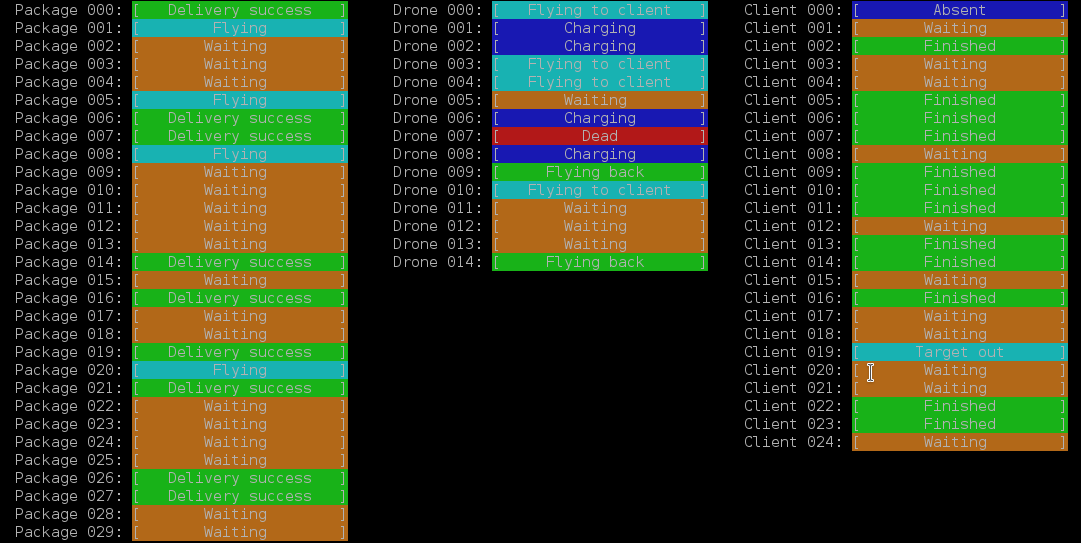
\includegraphics[width=\textwidth]{figures/UI1}
						\caption{Interface utilisateur: en cour d’exécution}
						\label{fig:UIrunning}
					\end{figure}
					Plusieurs états sont possible pour chaque type d'élément, exemples avec la figure \ref{fig:UIrunning}:
					\begin{itemize}
						\item Le paquet 000 a bien été livré
						\item Le paquet 001 est en vol
						\item Le paquet 002 est en attente d’être livré
						\item Le drone 000 est en vol vers le client
						\item Le drone 001 est en charge
						\item Le drone 005 est en attente (soit il attend qu'un paquet lui soit attribué soit il attend la fin de journée car les paquets restant sont trop lourd ou les clients trop loin pour lui)
						\item Le drone 007 est mort suite a un incident technique
						\item Le drone 009 est en vol vers le vaisseau mère après une livraison réussie
						\item Le client 000 est absent lors de sa livraison
						\item Le client 001 attend sa livraison
						\item Le client 002 a reçut tout ces paquets
						\item Le client 019 a sortit sa cible pour l'arrivée du drone
					\end{itemize}
					Tout au long de l’exécution du programme les différents acteurs du programme envoient des messages au dashboard pour prévenir de leur état jusqu’à la fin du programme ou chaque acteur est dans un état terminal comme visible sur la figure \ref{fig:UIend}.
					\begin{figure}[H]
						\centering
						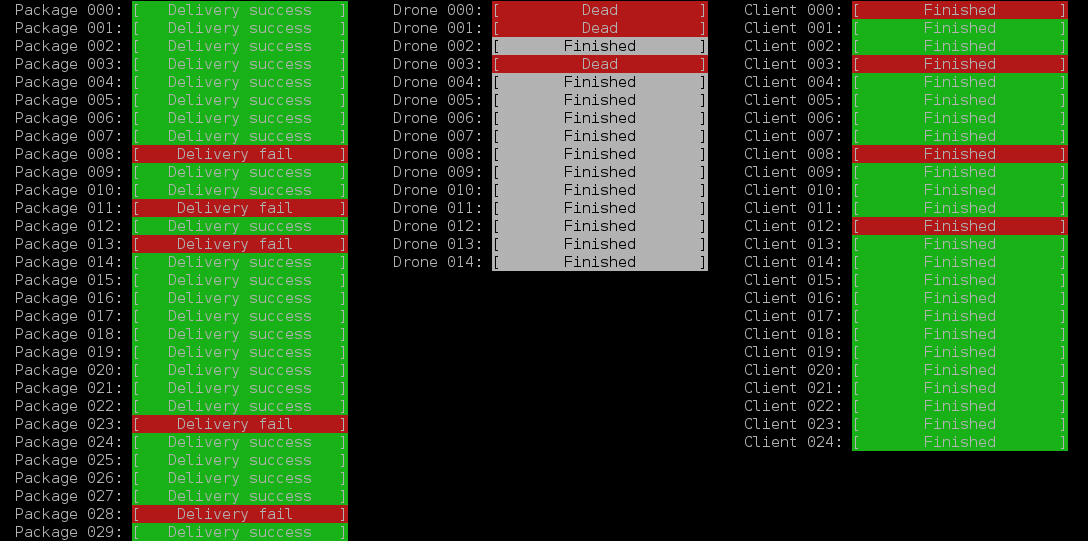
\includegraphics[width=\textwidth]{figures/UI2}
						\caption{Interface utilisateur: fin d’exécution}
						\label{fig:UIend}
					\end{figure}
					Les états finaux sont:
					\begin{itemize}
						\item Pour les paquets: livraison réussit ou échouée
						\item Pour les drones: journée finit ou mort
						\item Pour les clients: finit avec ayant reçut tout ces paquets ou finit avec des paquets manquants (limite d'essai atteint ou détruit avec la mort d'un drone)
					\end{itemize}
				\p{Configuration}
					Le dashboard est configurable, tout les messages d'état et les couleurs sont changeables. De plus le dashboard s'adapte dynamiquement a la taille de la console qui peut être redimensionnée au cour de l’exécution. En fonction de la largeur de la consule les élément s’afficheront sur 3 ou 1 colonne.
	\section{Utilisation}
		\subsection{Compilation}
			\subsubsection{Configuration}
				\TODO{pédantic}
				\TODO{Norme POSIX magique}
				\TODO{Prérequis: version min de gcc}
			\subsubsection{Makefile}
				Le \textit{Makefile} se charge de compiler d'abord la librairie \textit{ConsoleControl} puis de compiler le projet en liant cette dernière. Un \textit{Makefile} s'utilise avec le programme Make, pour plus d'informations sur Make voir \href{https://www.gnu.org/software/make/}{le site de gnu}.\\
				Le \textit{Makefile} se configure grace aux variables définies dans les deux premières sections, la configuration de base fournie est celle pour un OS Linux standard utilisant les commandes du shell et gcc.
				\begin{upmcaution}
					Compiler en \textbf{debug} pour tester est déconseillé car le logeur et le dashboard vont s'afficher en même temps, rendant le tout illisible.
				\end{upmcaution}
				\paragraph*{Flags utilisé (gcc)}
					\begin{itemize}
						\item Flags de version POSIX:
							\begin{lstlisting}[breaklines=true,breakatwhitespace=true,breakindent=0pt,columns=fixed,keepspaces=true,frame=single,basicstyle=\footnotesize\sffamily]
-D_POSIX_C_SOURCE=200112L\end{lstlisting}
							On définit \textit{\_POSIX\_C\_SOURCE} pour utiliser la version \textit{200112L} de la norme POSIX.
						\item Flags de warning:
							\begin{lstlisting}[breaklines=true,breakatwhitespace=true,breakindent=0pt,columns=fixed,keepspaces=true,frame=single,basicstyle=\footnotesize\sffamily]
-pedantic -pedantic-errors -Wall -Wcast-align -Wcast-qual -Wconversion -Wdisabled-optimization -Wdouble-promotion -Wextra -Wfloat-equal -Wformat -Winit-self -Winvalid-pch -Wlogical-op -Wmain -Wmissing-declarations -Wmissing-include-dirs -Wpointer-arith -Wredundant-decls -Wshadow -Wswitch-default -Wswitch-enum -Wundef -Wuninitialized -Wunreachable-code -Wwrite-strings\end{lstlisting}
							Pour plus d'information voir les \href{https://gcc.gnu.org/onlinedocs/gcc/Warning-Options.html}{options de warning gcc}.
					\end{itemize}
				\p{Compilation}
					Plusieurs cibles sont définies:
					\begin{description}
						\item[help] Affiches les cibles définit et leur effet
						\item[silent] Cible par défaut, équivalent a \texttt{make --silent all}
						\item[all] Compile le projet
						\item[debug] Compile le projet en debug en activant le logeur
						\item[clean] Supprime tous les fichiers et dossiers générés par le \textit{Makefile}
					\end{description}
					Pour appeler une cible:
					\begin{lstlisting}[breaklines=true,breakatwhitespace=true,breakindent=0pt,columns=fixed,keepspaces=true,frame=single,basicstyle=\footnotesize\sffamily]
$ make <cible>\end{lstlisting}
					Pour simplement compiler le projet:
					\begin{lstlisting}[breaklines=true,breakatwhitespace=true,breakindent=0pt,columns=fixed,keepspaces=true,frame=single,basicstyle=\footnotesize\sffamily]
$ make\end{lstlisting}
					Pour supprimer tous les fichiers et dossiers générés par le \textit{Makefile}:
					\begin{lstlisting}[breaklines=true,breakatwhitespace=true,breakindent=0pt,columns=fixed,keepspaces=true,frame=single,basicstyle=\footnotesize\sffamily]
$ make clean\end{lstlisting}
		\subsection{Exécution}
			\subsubsection{Paramètres}
				\TODO{Fichiers de config a passer en paramètres}
				\TODO{Fichiers par défaut et de test fournis}
			\subsubsection{Tests}
				\TODO{Valgrind}
\end{document}
